\documentclass[11pt]{article}
\usepackage{amsmath}
\usepackage{amssymb}
\usepackage{amsthm}
\usepackage{tikz}
\usepackage{geometry}
\geometry{margin=1in}

\DeclareMathOperator*{\argmax}{arg\,max}

\title{Deriving DT Loss with Simple Example}
\author{}
\date{}

\begin{document}
\maketitle

\section{Setup}
Let's derive DT loss with simple example:

We have a two frame video: $X_1, X_2$

Each frame has a noise level:
$K \sim \text{Uniform}(0, K)$ where 0 is no noise, $K$ is full.

So $X_1^{K_1}, X_2^{K_2}$ are the two frames with their noise levels $K_1, K_2$ respectively.

\section{Objective}
Let us define our goal:
\begin{align}
\argmax_\theta \mathbb{E}_{X_1^0, X_2^0 \sim p_{\text{data}}} \left[ \ln(p_\theta(X_1^0, X_2^0)) \right]
\end{align}

We derive a surrogate objective via the ELBO:
\begin{align}
\mathbb{E}_{X_1^0, X_2^0} \left[ \ln(p_\theta(X_1^0, X_2^0)) \right]
\end{align}

\begin{align}
= \mathbb{E}_{X_1^0, X_2^0} \left[ \ln \int p_\theta(X_1^0, X_2^0, X_1^{i:K}, X_2^{i:K}) dX_1^{i:K} dX_2^{i:K} \right]
\end{align}

Let's assume a Gaussian noising process:
\begin{align}
q(X_i^k | X_i^0) &\sim \alpha_K X_i^0 + \beta_K \epsilon, \quad \epsilon \sim \mathcal{N}(0, I) \\
&\sim \mathcal{N}(\alpha_K X_i^0, \beta_K I)
\end{align}

\begin{align}
&= \mathbb{E}_{X_1^0, X_2^0} \left[ \ln \int p(X_1^{0:K}, X_2^{0:K}) \cdot \frac{q(X_1^{1:K}, X_2^{1:K} | X_1^0, X_2^0)}{q(X_1^{1:K}, X_2^{1:K} | X_1^0, X_2^0)} dX_1^{1:K} dX_2^{1:K} \right] \\
&= \mathbb{E}_{X_1^0, X_2^0 \sim p_{\text{data}}} \left[ \ln \mathbb{E}_{X_1^{1:K}, X_2^{1:K} \sim q(\cdot | X_1^0, X_2^0)} \left[ \frac{p(X_1^{0:K}, X_2^{0:K})}{q(X_1^{1:K}, X_2^{1:K} | X_1^0, X_2^0)} \right] \right] \\
&\geq \mathbb{E}_{X_1^0, X_2^0 \sim p_{\text{data}}, X_1^{1:K}, X_2^{1:K} \sim q(\cdot | X_1^0, X_2^0)} \left[ \ln \left[ \frac{p(X_1^{0:K}, X_2^{0:K})}{q(X_1^{1:K}, X_2^{1:K} | X_1^0, X_2^0)} \right] \right]
\end{align}

\begin{align}
p(X_1^{0:K}, X_2^{0:K}) = p(X_1^K, X_2^K) \prod_{i \in \tau} p(T_{i-1} | T_i), \quad \tau \sim \text{Traj}(2,K)
\end{align}

where $T_i = (X_1^{K_i}, X_2^{K_i})$, $T_0 = (X_1^0, X_2^0)$, $T_K = (X_1^K, X_2^K)$.

Traj$(2, K)$ is the set of all trajectories on a 2-dimensional cube with $K$ delimiters. From 0 vertex to the opposite vertex.

\begin{align}
= \mathbb{E}_{X_1^{0:K}, X_2^{0:K}} \left[ \ln p(X_1^K, X_2^K) + \sum_{i \in \text{Traj}(2,K)} \ln \left( \frac{p(T_{i-1} | T_i)}{q(T_{i-1} | T_i)} \right) \right]
\end{align}

\begin{align}
= \mathbb{E}_{X_1^{0:K}, X_2^{0:K}} \left[ \ln p(X_1^K, X_2^K) \right] + \sum_{i \in \text{Traj}(2,K)} \mathbb{E}_{T_{i-1}, T_i} \left[ \ln \left( \frac{p(T_{i-1} | T_i)}{q(T_{i-1} | T_i) \cdot q(T_i)} \right) \right]
\end{align}

We take all constants w.r.t $p$ out:
\begin{align}
= \mathbb{E}_{X_1^K, X_2^K} \left[ \ln p(X_1^K, X_2^K) \right] + \sum_{i \in \text{Traj}(2,K)} \mathbb{E}_{T_{i-1}, T_i} \left[ \ln \left( \frac{p(T_{i-1} | T_i)}{q(T_{i-1} | T_i)} \right) \right]
\end{align}

\begin{align}
= \mathbb{E}_{X_1^K, X_2^K} \left[ \ln p(X_1^K, X_2^K) \right] + \sum_{i \in \text{Traj}(2,K)} D_{KL}(q(T_{i-1} | T_i) || p(T_{i-1} | T_i))
\end{align}

We create indicator indicating if $X_1^{K_1}, X_2^{K_2} \leftrightarrow X_1^{K_1'}, X_2^{K_2'}$ is included in the trajectories of interest.

$\mathbb{I}(X_1^{K_1}, X_2^{K_2} \leftrightarrow X_1^{K_1'}, X_2^{K_2'})$

We can introduce probabilities of different trajectories: e.g. $p_\pi$

This modifies our loss by now having a weighted sum over the $D_{KL}$ of our trajectories:
\begin{align}
\mathbb{E}_{i \in \text{Traj}(2,K)_\pi} \left[ D_{KL}(q(T_{i-1} | T_i) || p(T_{i-1} | T_i)) \right]
\end{align}

Now we sum over ALL possible $2^K$ trajectories:
\begin{align}
= \sum_{i \in \text{Traj}(2,K)_\pi} p(\pi) \cdot D_{KL}(q(T_{i-1} | T_i) || p(T_{i-1} | T_i))
\end{align}

\section{Generalizing to the n-frame case}

\begin{align}
\sum_{i \in \text{Traj}(n,K)} P(T_i \rightarrow T_i') D_{KL}(q(T_{i-1} | T_i) || p(T_{i-1} | T_i))
\end{align}

In DF we have $P(T_{i-1} \rightarrow T_i)$:
\begin{align}
= \mathbb{I}\left( \left( K_1^{T_i}, K_2^{T_i} \right) - \left( K_1^{T_i-1}, K_2^{T_i-1} \right) = \left( K_1^{T_i}, K_2^{T_i} - 1 \right) \right)
\end{align}

But indicator didn't draw all arrows, but indicator of all trajectories with
\begin{align}
= (K-1)^n
\end{align}
but this should not be the case if we never double back and assign equal probability to each trajectory (you expect transitions of states near the diagonal to be weighted more by binomial...).

\section{DF Weights}

DF weights should be:

\begin{center}
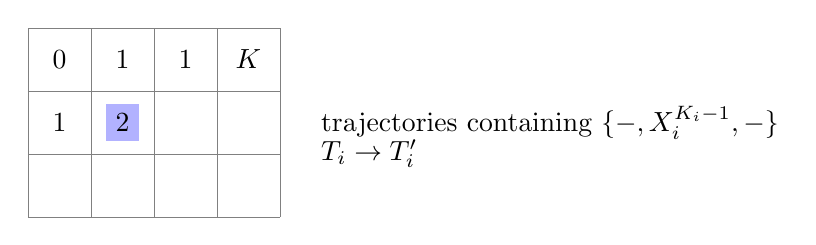
\begin{tikzpicture}[scale=0.8]
\draw[step=1cm,gray,very thin] (0,0) grid (4,3);
% Labels on top row
\node at (0.5,2.5) {0};
\node at (1.5,2.5) {1};
\node at (2.5,2.5) {1};
\node at (3.5,2.5) {$K$};
% Labels on second row
\node at (0.5,1.5) {1};
\node[fill=blue!30] at (1.5,1.5) {2};
% Text to the right
\node[anchor=west] at (4.5,1.5) {trajectories containing $\{-, X_i^{K_i-1}, -\}$};
\node[anchor=west] at (4.5,1) {$T_i \rightarrow T_i'$};
\end{tikzpicture}
\end{center}

We have:
\begin{align}
\begin{pmatrix}
K_1 + \cdots + K_n - 1 \\
K_1, K_2, \cdots, K_i - 1, \cdots, K_n
\end{pmatrix} + \begin{pmatrix}
(K - K_1) + \cdots + (K - K_n) \\
K - K_1, \cdots, K - K_n
\end{pmatrix}
\end{align}

\begin{align}
= \begin{pmatrix}
n \cdot K \\
K, K, \cdots, K
\end{pmatrix}_{n \text{ times}}
\end{align}

TF is encapsulated in this framework too.

TF weights should be a constant traversing the edge of the cube from frame 1 $\rightarrow$ frame 2 $\rightarrow$ ... denoising which is:

\begin{align}
\mathbb{I}\left( \left\{ X_1^0, X_2^0, \ldots, X_i^{K_i}, X_{i+1}^K, \ldots, X_n^K \right\} \rightarrow \left\{ X_1^0, X_2^0, \ldots, X_i^{K_i-1}, X_{i+1}^K, \ldots, X_n^{1K} \right\} \right)
\end{align}

i.e. pick any frame $i$, every frame to the left should be clean, every frame to the right should be full noise, and the transition should be denoising the $i$th frame by 1 noise level.

But might seem like it is not what it is.

Transformers will simultaneously submit predictions for every frame, but in the run case, we just iterate through all frames (in any order) and denoise them by 1 step.

\begin{center}
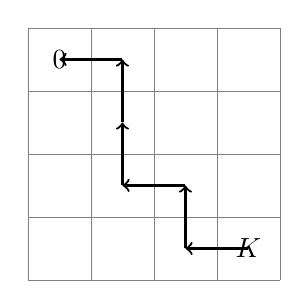
\begin{tikzpicture}[scale=0.8]
\draw[step=1cm,gray,very thin] (0,0) grid (4,4);
% Step pattern
\draw[->,thick] (3.5,0.5) -- (2.5,0.5);
\draw[->,thick] (2.5,0.5) -- (2.5,1.5);
\draw[->,thick] (2.5,1.5) -- (1.5,1.5);
\draw[->,thick] (1.5,1.5) -- (1.5,2.5);
\draw[->,thick] (1.5,2.5) -- (1.5,3.5);
\draw[->,thick] (1.5,3.5) -- (0.5,3.5);
\node at (3.5,0.5) {$K$};
\node at (0.5,3.5) {0};
\end{tikzpicture}
\end{center}

If we do architecture such as the transformer that predicts all frames at once, then our possible trajectories are just diagonals:

\begin{center}
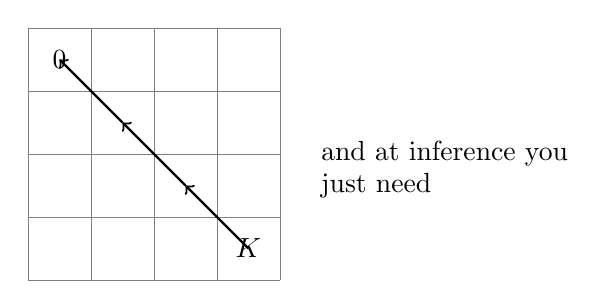
\begin{tikzpicture}[scale=0.8]
\draw[step=1cm,gray,very thin] (0,0) grid (4,4);
% Diagonal arrows
\draw[->,thick] (3.5,0.5) -- (2.5,1.5);
\draw[->,thick] (2.5,1.5) -- (1.5,2.5);
\draw[->,thick] (1.5,2.5) -- (0.5,3.5);
\node at (3.5,0.5) {$K$};
\node at (0.5,3.5) {0};
\node[anchor=west] at (4.5,2) {and at inference you};
\node[anchor=west] at (4.5,1.5) {just need};
\end{tikzpicture}
\end{center}

\begin{center}
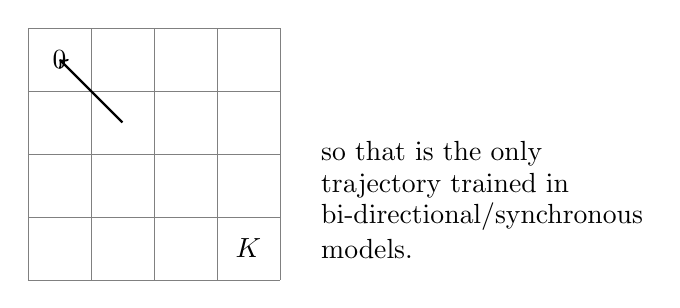
\begin{tikzpicture}[scale=0.8]
\draw[step=1cm,gray,very thin] (0,0) grid (4,4);
% Single diagonal arrow
\draw[->,thick] (1.5,2.5) -- (0.5,3.5);
\node at (0.5,3.5) {0};
\node at (3.5,0.5) {$K$};
\node[anchor=west] at (4.5,2) {so that is the only};
\node[anchor=west] at (4.5,1.5) {trajectory trained in};
\node[anchor=west] at (4.5,1) {bi-directional/synchronous};
\node[anchor=west] at (4.5,0.5) {models.};
\end{tikzpicture}
\end{center}

\section{Deriving the Self-Forcing Objective and Training Algorithm}

Let's derive the self-forcing objective and training algorithm from the following:

Instead of $\argmax_\theta \mathbb{E}_{X \sim p_{\text{data}}} \left[ \ln(p_\theta(X)) \right]$,

we swap $p_{\text{data}}$ and $p_\theta$ to get:
\begin{align}
\argmax_\theta \mathbb{E}_{X_1^0, X_2^0 \sim p_\theta} \left[ \ln(p_{\text{data}}(X_1^0, X_2^0)) \right]
\end{align}

\begin{align}
= \argmax_\theta \mathbb{E}_{X_1^0, X_2^0 \sim p_\theta} \left[ \ln \int p_{\text{data}}(X_1^{0:K}, X_2^{0:K}) \cdot \frac{p_\theta(X_1^{1:K}, X_2^{1:K} | X_1^0, X_2^0)}{p_\theta(X_1^{1:K}, X_2^{1:K} | X_1^0, X_2^0)} dX_1^{1:K} dX_2^{1:K} \right]
\end{align}

\begin{align}
= \argmax_\theta \mathbb{E}_{X_1^0, X_2^0 \sim p_\theta, } \left[ \ln \mathbb{E}_{X_1^{1:K}, X_2^{1:K} \sim p_\theta(\cdot | X_1^0, X_2^0)} \left[ \frac{p_{\text{data}}(X_1^{0:K}, X_2^{0:K})}{p_\theta(X_1^{1:K}, X_2^{1:K} | X_1^0, X_2^0)} \right] \right]
\end{align}

\begin{align}
\geq \argmax_\theta \mathbb{E}_{X_1^{0:K}, X_2^{0:K} \sim p_\theta} \left[ \ln \left( \frac{p_{\text{data}}(X_1^{0:K}, X_2^{0:K})}{p_\theta(X_1^{1:K}, X_2^{1:K} | X_1^0, X_2^0)} \right) \right]
\end{align}

\end{document}